\section{Punto de Vista de Mapa de Recurso}

El punto de vista del mapa de recursos permite al arquitecto comercial crear una descripción general estructurada de los recursos de la empresa. Un mapa de recursos generalmente muestra dos o tres niveles de recursos en toda la empresa. Puede, por ejemplo, utilizarse como mapa de calor para identificar áreas de inversión. En algunos casos, un mapa de recursos también puede mostrar relaciones entre los recursos y las capacidades a las que están asignados.

\subsection{Modelo de Mapa de Recurso}
\begin{figure}[h!]
	\centering
	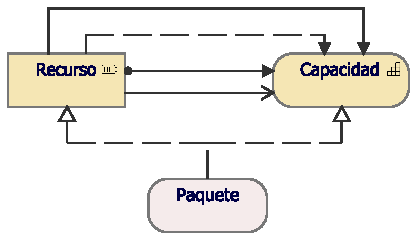
\includegraphics[width=.5\linewidth]{imgs/caso/MapaRecurso.pdf}
	\caption{Modelo Mapa de Recurso}
\end{figure}

El punto de vista del mapa de recursos proporciona una descripción estructurada de los recursos de la empresa.

\newpage

\subsection{Caso de Mapa de Recurso}

\subsubsection{Resultado 1: Mejores Investigadores e Investigaciones}

\begin{figure}[h!]
	\centering
	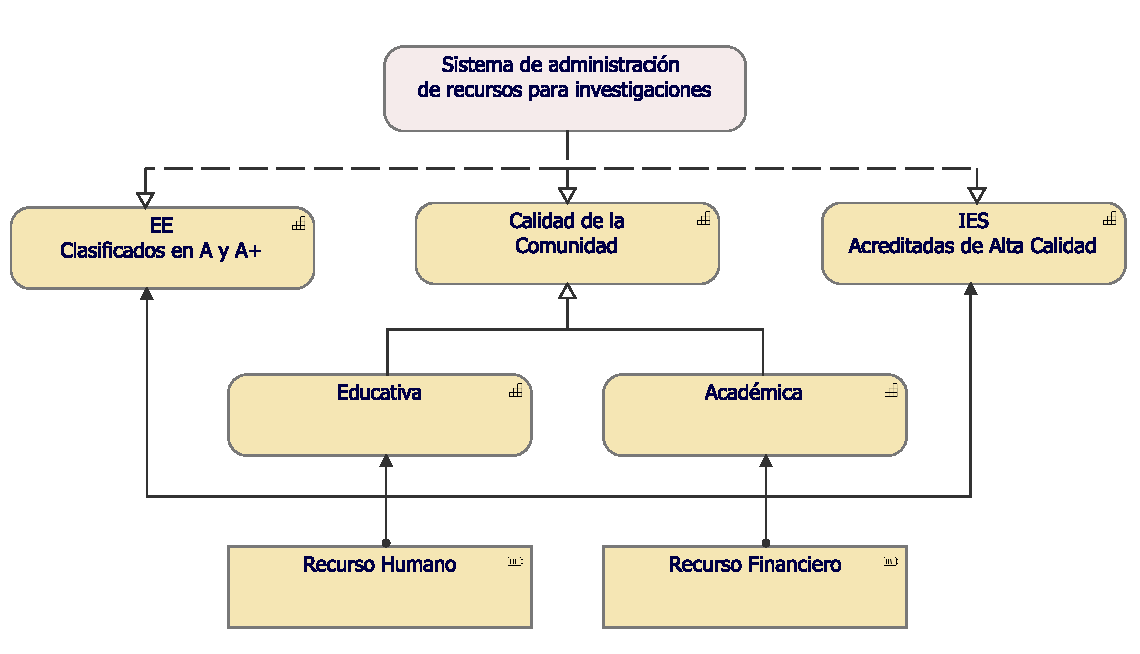
\includegraphics[width=1\linewidth]{imgs/modelo/estrategia/mapa/mapa_recurso.pdf}
	\caption{Caso Mapa de Recurso}
\end{figure}

Para dar alcance a las capacidades de calidad de la comunidad, IES Acreditadas de Alta Calidad y EE Clasificados en A y A+ basadas en habilidades dadas por el resultado de Mejores Investigadores e Investigaciones, se pretende construir un sistema que administre de manera optima los recursos para realizar nuevas investigaciones dando lugar a un crecimiento exponencial de nuevos investigadores.

\clearpage
\subsubsection{Resultado 2: Generación de Estudiantes de Alta Calidad}

\begin{figure}[h!]
	\centering
	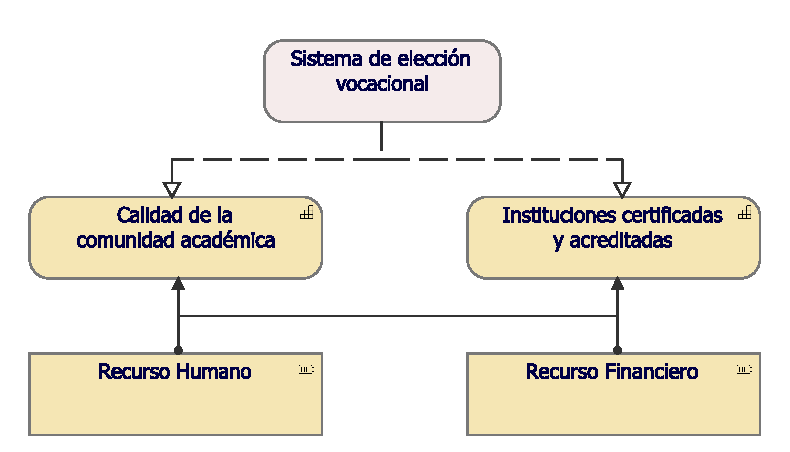
\includegraphics[width=.8\linewidth]{imgs/modelo/estrategia/mapa/mapa_recurso_2.pdf}
	\caption{Caso Mapa de Recurso}
\end{figure}

Para garantizar la generación de estudiantes de calidad es necesario implantar nuevos sistemas que ayudan a elegir de mejor manera la vocación que tendrán en el futuro los estudiantes. Buscando así que el estudiante se acerque a las diferentes carreras o áreas del conocimiento sin sentir presión por parte de ningún ente, que aquella vocación escogida por el estudiante sea totalmente de su agrado y gusto; formando estudiantes que lleven la educación de calidad no por obligación sino por interés propio.